\newpage
\rhead{Галибов}
\subsection{Теорема Больцано--Коши о промежуточном значении}

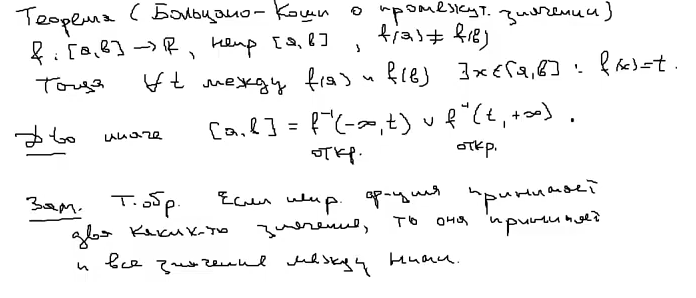
\includegraphics[scale=1.0]{Images/Больцано - Коши.png}





\newpage
\subsection{Теорема о бутерброде}
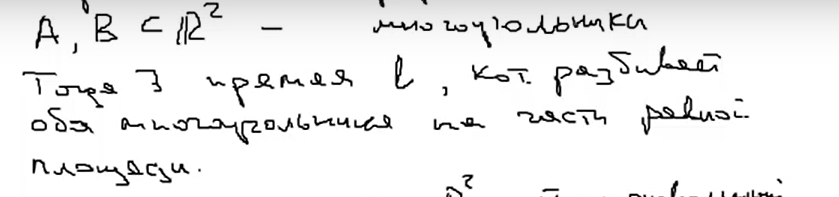
\includegraphics[scale=0.7]{Images/Бутерброд.png}


Доказательство:\\

Лемма: 

$A \subset R^2$, V - произвольный вектор. Тогда $\exists$ прямая с направлением вектора V, делящая фигуру на части одинаковой площади.\\

Доказательство Леммы: \\

Пусть $A \subset [a,b]\times[c,d]$. Не умоляя общности пусть $[a,b] \not \parallel V$. Где $[a,b]$ - часть оси OX.
Рассмотрим координату на оси ОХ 
$\forall t$ $f(t) = S_l (t) - S_r (t)$ 
$f(a) = -S$, а $f(b) = S$.
f - непрерывна: $|f(t_1) - f(t_2)|$ $\leq$ 2 * площадь слоя фигуры между $t_1$ и $t_2$ $\leq$ $2*(d - c)*|t_1 - t_2|$
По теореме Больцано-Коши о промежуточном значении $\exists t_0$ : $f(t_0) = 0$\\


Доказательство Теоремы: \\

$\forall \phi \in [0,2*\pi]$ построим по лемме прямую направленную под углом $\phi$ к оси OX. Она делит A на равновеликие части. $g(\phi) = S^B_l(\phi) - S^B_r(\phi)$. (Площади фигуры B). \\

1 утверждение (очевидное) (для получения периодичности)

$g(\phi + \pi) = -g(\phi)$

2 утверждение (g - непрерывно)

% запиши 1/2 через frac
$g(\phi_1) - g(\phi_2) \leq 4* 1/2 * d^2 * |sin(\phi_1 - \phi_2)|$, где d - диагональ стола.
По теореме Больцано-Коши о промежуточном значении все получается.
% Хотелось бы вывод получше


\newpage
\subsection{Теорема о сохранении промежутка}

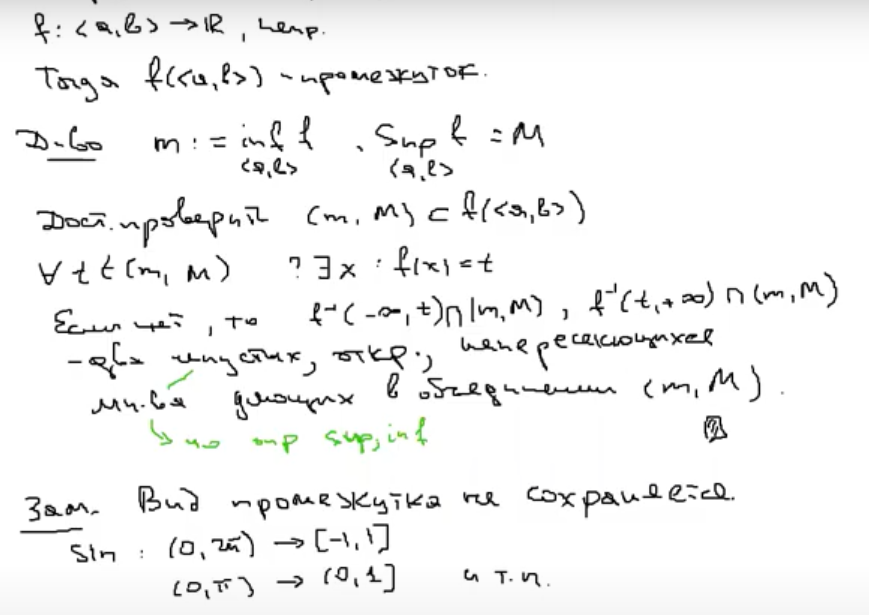
\includegraphics[scale=0.7]{Images/Сохранение промежутка.png}



\newpage
\subsection{Теорема Больцано--Коши о сохранении линейной связности}

Определение: Пусть $Y$ - метрическое пространство и $E \subset Y$.

E - линейно связное если $\forall A,B \in E \  \exists$ путь $c:[a,b] \to E$ - непрерывный, такой что $c(a) = A, c(b) = B$.\\

% непонятно - лучше привести конкретный пример пути
Пример 1 - круг в $\R^2$ - линейно связный потому что выпуклый.\\
$g :[0,1] \to \R^2$\\
$t \to A + t(B - A)$\\

% это не линейно связное мн-во и нужно доказать, почему
Пример 2 - $A \subset \R^2$   
$A = ({0} \times [-1, 1]) \cup \{(x, sin{\frac{1}{x}}) : x \in \R, x \not = 0\}$\\

Теорема :

X - линейное связное множество. $f : X \to Y$ (на Y - сюръекция) - непрерывно.
Тогда Y - линейное связно.\\

Доказательство :

$A, B \in Y$ подберем $U,V \in X$ : $f(U) = A, f(V) = B$;

Соединим U и V путем  с (т.е. возьмем $c : [a, b] \to X, c(a) = U, c(b) = V$). Тогда
% требует пояснения о непрерывности композиции
композиция f и c соединяет точки A и B.

\newpage
\subsection{Описание линейно связных множеств в $\R$}
% зачем тут определение и примеры, когда они есть на предыдущей странице
Определение: Пусть $Y$ - метрическое пространство и $E \subset Y$.

E - линейно связное если $\forall A,B \in E \exists$ путь $c:[a,b] \ to E$ - непрерывный, такой что $c(a) = A, c(b) = B$.\\

Пример 1 - круг в $\R^2$ - линейно связный потому что выпуклый.\\
$g :[0,1] \to \R^2$\\
$t \to A + t(B - A)$\\

Пример 2 - $A \subset \R^2$   $A = ({0} * [-1, 1]) \cup {(x, sin{\frac{1}{2}} : x \in \R, x \not = 0)}$\\

Теорема : 

В $\R^1$ линейно связыми множествами являются только промежутки.\\

Доказательство : 

% оформление не оч
В утверждении спрятана $\leftrightarrow$.
E - промежуток $\rightarrow$ E - линейно связно. Очевидно.
E - линейно связно. $m = \inf E, M = \sup E$. Проверим, что $(m, M)\subset E$.
Пусть $t \in (m, M)$: $t \not \in E$.
% почему такие А и В существуют?
Возьмем $A \in E : A < t$, $B \in E : t < B$

Тогда $\not\exists$ пути из A в B. (Если бы существовал такой путь, 
% почему? поясни
то в некоторой точке $d \in (a,b) : c(d) = t$).
